%%%%%%%%%%%%%%%%%%%%%%%%%
% Response to reviewer Template
% C. Ocampo-Martinez (2014)
%%%%%%%%%%%%%%%%%%%%%%%%%

\documentclass[11pt]{article}

\usepackage[letterpaper,left=3.0cm,right=3.0cm,top=2.0cm,bottom=2.0cm]{geometry}
\setlength{\parskip}{2ex}
\setlength{\parindent}{0ex}

\usepackage[english]{babel}
\usepackage{times, epsfig, subfigure, psfrag, amssymb, amsmath, amsbsy, amsfonts}
\usepackage{graphics}
\usepackage{tabularx}
\usepackage[utf8]{inputenc}
\usepackage[T1]{fontenc}
%\usepackage{url,soul,ulem}
\usepackage{stfloats}
\usepackage{array, color}
\usepackage{bm}
\usepackage{tabularx}
\usepackage{fancyhdr}
\usepackage{datetime,enumitem}
\usepackage{algorithmic}
\usepackage{cite}
\usepackage[dvipsnames]{xcolor}
\usepackage{algorithm}
\usepackage[normalem]{ulem}
\usepackage{amssymb}
\usepackage{amsmath}
\usepackage{empheq}
\setlist[enumerate]{label=\alph*),topsep=0ex,parsep=0ex,partopsep=0ex}


\newtheorem{definition}{Definition}%{\itshape}{\bfseries}
\newtheorem{example}{Example}%{\it}{}
\newtheorem{corollary}{Corollary}%{\it}{}
\newtheorem{proposition}{Proposition}%{\it}{}
\newtheorem{lemma}{Lemma}%{\it}{}
\newtheorem{theorem}{Theorem}%{\it}{}
\newtheorem{remark}{Remark}%{\it}{}
\newtheorem{assumption}{Assumption}%{\it}{}
%\newenvironment{proof}[1][Proof]{\noindent\textbf{#1.} }{\ \rule{0.5em}{0.5em}}
%\newcommand{\proof}{\vspace{1mm}\noindent{\it Proof.}\quad}
%\def\qed{\quad{$\square$}} 

%\textwidth=6.3in
%\textheight 9in 
%\setlength{\topmargin}{-0.5in}
%\setlength{\oddsidemargin}{0.1in} 
%\setlength{\evensidemargin}{0.1in}
%%%%%%%%%%%%%%%%%%%%%%%%%%%%%%%%%%
\def\an#1{{{\bf \color{blue}#1}}}
\def\o{{\bm{\omega}}}
\def\vmean{v^{\rm mean}}
\def\vmax{v^{\rm max}}	
\def\e{\epsilon}
\newcommand{\todo}[1]{\vspace{5 mm}\par \noindent \marginpar{\textsc{ToDo}}
	\framebox{\begin{minipage}[c]{0.9 \textwidth} \tt #1
	\end{minipage}}\vspace{5 mm}\par}

% Boldsymbols, mathcal, mathbb
\newcommand{\bs}{\boldsymbol}
\newcommand{\mc}{\mathcal}
\newcommand{\bb}{\mathbb}
\newcommand{\R}{\bb R}

\DeclareMathAlphabet{\mathbbmsl}{U}{bbm}{m}{sl}
\newcommand{\bbi}{\mathbbmsl}
%norm
\newcommand{\norm}[1]{\left\|#1\right\|}

% Operators and notations
\newcommand{\dom}{\operatorname{dom}}
\newcommand{\iP}{\mathcal{P}}
\newcommand{\B}{\mathcal{C}}
\newcommand{\red}{\textcolor{red}}
\newcommand{\blue}{\textcolor{blue}}
\newcommand{\green}{\textcolor{green}}
\newcommand{\argmin}{\operatorname{argmin}}
\newcommand{\mini}{\operatorname{minimize}}
\newcommand{\Proj}{\mathrm{Proj}}
\newcommand{\fix}{\mathrm{fix}}
\newcommand{\proj}{\mathrm{proj}}
\newcommand{\prox}{\mathrm{prox}}
\newcommand{\Id}{\mathrm{Id}}
\newcommand{\Res}{\operatorname{J}}
\newcommand{\diag}{\operatorname{diag}}
\newcommand{\blkdiag}{\operatorname{blkdiag}}
\newcommand{\col}{\operatorname{col}}
\newcommand{\zer}{\operatorname{zer}}
\newcommand{\nulls}{\operatorname{Null}}
\newcommand{\range}{\operatorname{Range}}
\newcommand{\dist}{\mathrm{dist}}
\newcommand{\nc}{\mathrm{N}}
\newcommand{\0}{\mathbf{0}}
\newcommand{\1}{\mathbf{1}}
\newcommand{\half}{^1\hspace*{-.1em}/_2}
\newcommand{\gph}{\operatorname{gph}}
%Roman numbers
\newcommand{\rmnum}[1]{\romannumeral #1}
\newcommand{\Rmnum}[1]{\expandafter\@slowromancap\romannumeral #1@}
\newcommand{\eod}{\ensuremath{\hfill\Box}}
\newcommand{\qedd}{\ensuremath{\hfill \blacksquare}}



% Add time and date to pages
% *****************************************
%\cfoot[\thepage]{\thepage}
%\chead[]{}\lhead[\currenttime]{\currenttime}\rhead[\today]{\today}
%\pagestyle{fancy}
% *****************************************
\usepackage[nobottomtitles*]{titlesec}
\titleformat{\section}%
    {\bfseries\large}{}{0.0em}{}[]%
\titlespacing*{\section}%
    {-0.5cm}{2.5ex plus 0.2ex minus 0.2ex}{0.5ex plus 0.2ex minus 0.2ex}%

\usepackage{ifthen}
\newcommand{\query}[2][]{
    \ifthenelse{\equal{#1}{}}{}{\textbf{#1:}~}\emph{#2}\\[0.1em]}
\newcommand{\ans}[1]{\textbf{Answer:~}
    \ifthenelse{\equal{#1}{}}{To be answered!}{#1}}


% Use for adding comments according to the author (different color)
% CUSTOMIZE
%\newcommand{\XXX}[1]{\textcolor{red}{#1}}
\newcommand{\com}[1]{\textcolor{blue}{#1}}
\newcommand{\edit}[1]{\color{blue}{#1 }\color{black} }
\newcommand{\comment}[1]{\textcolor{red}{[#1]}}
%\newcommand{\XX}[1]{\textcolor[rgb]{0,0.5,0}{#1}}
%\newcommand{\XXXX}[1]{\textcolor[rgb]{0.50,0.00,0.50}{#1}}


\title{Authors' response}
\date{}
\begin{document}
%\maketitle

\begin{center}
\textbf{\Large Authors' response}
\end{center}
\vspace{0.5cm}
\noindent

\textbf{Ms. Ref. No.: TSG-01404-2021}  \\
\textbf{Title: Operationally-Safe Peer-to-Peer Energy Trading in Distribution Grids: A Game-Theoretic Market-Clearing Mechanism}   \\
\textbf{Authors: G. Belgioioso, W. Ananduta, S. Grammatico, and C. Ocampo-Martinez}   \\
\textbf{Journal: IEEE Transactions on Smart Grid}  

%\vspace{1cm}

\setcounter{page}{1}

% ADD HERE PREAMBLE TEXT
The authors would like to thank the Reviewers and the Associate Editor for their comments, which have helped us to improve the manuscript. We do hope that all the points raised have been addressed. {To help reviewing the revised manuscript,} the points have been divided up and marked AE, R1, R2, R3, and R4, for comments from Associate Editor, Reviewers 1, 2, 3, and 4, respectively. When appropriate, the corresponding marks can be found within the manuscript and the modifications according to the comments are highlighted in \textcolor{blue}{blue}. In addition, the cross references of equation labels, as mentioned by the reviewers and used in the answers, are adapted based on the revised manuscript. %We have also removed some intermediate steps in the derivation of some (in)-equalities and displayed some equations in different forms to meet the page limit. These parts are highlighted in \textcolor{magenta}{magenta}.%Additionally, in order to adjust the contents into a technical note, we have streamlined some parts of the paper, which are highlighted in \textcolor{magenta}{magenta}.


\section*{Answers to Associate Editor}

\query[AE-1]{This paper proposes a generalized Nash game model for P2P energy trading in a distribution network considering network constraints and DNO. A distributed algorithm is developed to seek the equilibrium of the game. The topic is relevant and timely. However, the reviewers raised some concerns. The authors should carefully consider all the comments and make a corresponding improvement. } 
\ans{We thank the Associate Editor for handling our manuscript and providing positive comments. We have addressed all the comments from the reviewers and revised the manuscript accordingly.}


\newpage
\section*{Answers to Reviewer 1}


\query[R1-1]{This paper proposed a peer-to-peer energy market for prosumers as a generalized aggregative game. The paper is well written, and the research may be of value. The reviewer mainly concerns about the proposed algorithm.}
\ans{We thank the reviewer for the positive comment.}



\textit{The comments are as follows:}

\query[R1-2]{The feasibility of such scenarios still remains further discussions considering the capital costs of energy storage, interests conflicts of current electrical roles, and the engineering implementations involving such accurate models.}
\ans{We agree with the Reviewer. This work particularly shows how a distributed clearing mechanism that can be implemented in such scenarios as well as how peer-to-peer market scenarios in theory can be beneficial.}

\query[R1-3]{The charging and discharging efficiency are not considered in (5), which is sometimes acceptable, but requires explanations.  }
\ans{In the first version of the manuscript, we did not consider the charging and discharging efficiency as we assume the simplest model of the storage since component model is not the main focus of this work. However, based on this reviewer comment, we now update the storage dynamics, which include the charging and discharging efficiencies. Therefore, for each storage unit, we consider two decision variables, i.e., the charging and discharging powers. The storage unit is now modeled as follows:}

\textit{``\edit{The battery charging and discharging profiles, $p_{i}^{\mathrm{ch}} = \col((p_{i,h}^{\mathrm{ch}})_{h\in \mc H})$ and $p_{i}^{\mathrm{ds}} = \col((p_{i,h}^{\mathrm{ds}})_{h\in \mc H})$, respectively, are constrained by the battery dynamics}}
%
\begin{equation}
%	\marginnote{\note{R1-3}\\ \note{R2-2}}
	\begin{aligned}
		\left.
		\begin{array}{c}
			\edit{	x_{i,h+1} =\eta_i^{\mathrm{st}} x_{i,h} +\frac{T_{\mathrm{s}}}{e^{\mathrm{cap}}_{i}}(\eta_i^{\mathrm{ch}} p_{i,h}^{\mathrm{ch}} -(\frac{1}{\eta_i^{\mathrm{ds}}})p_{i,h}^{\mathrm{ds}}),} \\[.2em]
			\underline{x}_i \leq x_{i,h+1} \leq \overline{x}_i, \\[.2em]
			\edit{	{p}_{i}^{\mathrm{ch}} \in [0,\overline{{p}}_{i}^{\mathrm{ch}}], \ \ {p}_{i}^{\mathrm{ds}} \in [0,\overline{{p}}_{i}^{\mathrm{ds}}],}
		\end{array}
		\hspace{-5pt} \right\} & \begin{matrix}
			\forall i \in \mc N^{\mathrm{st}}, \\ \forall h \in \mc H,
		\end{matrix} \\
		\edit{p_{i}^{\mathrm{ch}}= 0, \ \ p_{i}^{\mathrm{ds}}= 0,}\qquad \qquad & \forall i \notin \mc N^{\mathrm{st}},
	\end{aligned}
	\label{eq:x}
\end{equation}
\textit{where $x_{i,h} $ denotes the state of charge (SoC) of the storage unit at time $h \in \mc H$%
%\footnote{In \cite{atzeni2013}, the charging and discharging power are defined separately, which is actually a better representation. However, the optimal strategies that they produce satisfies the constraint that charging and discharging must be mutually exclusive (see footnote 1 in \cite{atzeni2013}). From other papers, they usually have boolean variables to ensure this constraint and we want to avoid that.}
, \edit{$\eta_i^{\mathrm{st}}, \eta_i^{\mathrm{ch}}, \eta_i^{\mathrm{ds}} \in (0,1]$ denote  the leakage coefficient of the storage, charging, and discharging efficiencies, respectively, while }  %$b_i~=~-\frac{T_{\mathrm{s}}}{e^{\mathrm{cap}}_{i}}$, with 
$T_{\mathrm{s}}$ and $e^{\mathrm{cap}}_{i}$ denote sampling time and maximum capacity of the storage, respectively. Moreover, $\underline{x}_i,\overline{x}_i  \in [0,1]$  denote the minimum and the maximum SoC of the storage unit of prosumer $i$, respectively, whereas $\edit{\overline p}^{\mathrm{ch}}_i \geq 0$ and $\edit{\overline p}^{\mathrm{ds}}_i \geq 0$ denote the maximum charging and discharging power of the storage unit. Finally, we denote by  $\mathcal{N}^{\mathrm{st}}\subseteq\mathcal{N}$ 	the set of prosumers that own a storage unit.''}

We have also modified our game formulation and proposed algorithm in Section III to take into account this storage model update.

\query[R1-4]{The energy loss of the distribution network is also not considered.}
\ans{We do not include energy loss of the distribution network in the current setup and leave it for future work. In this manuscript, we focus on the game-theoretic formulation of the interaction among prosumers and the network operator and show that the problem can be solved efficiently. For an extension that includes energy losses, we may impose to each prosumer an additional linear cost function that depends on the losses caused by trading and use linear model of power line losses as in \cite[Section II]{moret2020}.}

\query[R1-5]{The individual variables, coupled relationships for these energy roles, and the corresponding dual variables should be explained specifically, along with the whole framework structure for equilibrium. The rationalities of the framework is not clear. At least, the current presentation is hard to follow.  }
\ans{
\green{
In the revised paper, (i) we provided a detailed description of each individual variable along with an explanation of its function in the algorithm; (ii) we re-designed the main algorithm layout; and (iii) we included a paragraph to present the targeted class of equilibria considered. Please, refer to the margin notes (R1-5) in Section III for the relative changes and additions.
}
}

\query[R1-6]{The P2P trading prices are given parameters, which are quite unreasonable. In fact, the P2P prices are the key variable in most literature.}
\ans{In this manuscript, we want to consider the most general problem formulation of peer-to-peer markets available in the literature. Following \cite{sorin2019,lecadre2020,baroche2019b}, a linear trading cost function is introduced in the problem formulation for the purpose of product differentiation or preference prices. %Furthermore, \cite{baroche2019} also adds a trading tariff or transaction cost encoded as a 1-norm cost function. 
	Furthermore, we may set $c_{\{i,j\}}^{\mathrm{tr}}=0$, and thus only consider the dual variable associated with the reciprocity constraints (Eq. \red{(8b)} in the revised manuscript) as the shadow price of bilateral trading \cite[Section 2.4]{lecadre2020}. Indeed the proposed algorithm can handle any case where $c_{\{i,j\}}^{\mathrm{tr}} \geq 0$, for all $\{i,j\} \in \mc E$.}

 \query[R1-7]{The algorithm requires too many iterations, which leads to poor feasibility in real applications, especially in distributed environment. }
 \ans{
\green{The average computational time (obtained using a pc with Intel Xeon E5-2637 3.5 GHz processors and 128 GB of memory) for the parallel updates of each prosumer (i.e., Algorithm 2) is $t_{\text{avg}}^{\text{pro}} = 74.5$ milliseconds; while for the DNO update (i.e., Algorithm 3), the average computational time is $t_{\text{avg}}^{\text{DNO}} = 1.13$  seconds. 
%
 Hence, the total running time of the proposed market-clearing algorithm (Algorithm 1) implemented on a distributed system can be approximatively calculated as
\begin{align*}
\text{total computation time} = \text{\# iterations for convergence } \times (t_{\text{avg}}^{\text{pro}} + 	t_{\text{avg}}^{\text{DNO}}),
\end{align*}
which yields running times of less than 23 minutes. 
%
We consider this computational-time requirement reasonable for day-head or also for intra-day scheduling purposes. Moreover, we note that the total running time can be considerably reduced by (i) using provably-convergent accelerated versions of our market-clearing mechanism, that can be easily devised by exploiting the algorithmic framework in \cite[\S~IV-B]{belgioioso2020semi} and in practice reduce (potentially, halve) the total number of iterations for convergence;
(ii) designing a more efficient ad-hoc algorithm to solve the projection step in Algorithm 3 (i.e., Algorithm 3 (i)); (iii) using a more computationally-powerful hardware to perform the DNO central updates, namely, Algorithm 3. Finally, we note that the main algorithm is scalable with respect to the prosumer population size, namely, the number of iterations for convergence is not affected by the total number of prosumers in the network (see Figure \red{10}). Moreover, the computation time of the local updates is virtually also independent from the prosumer population size, for constant connectivity levels of the trading network. Therefore, the previous approximation remains valid independently from the market size.
} }


\newpage
\section*{Answers to Reviewer 2}

\query[R2-1]{This manuscript proposes a game model for P2P energy trading in a distribution network considering network constraints and the DNO agent. The game model is a generalized game in which agents have coupled objectives and constraints. A distributed algorithm is developed to seek the equilibrium of the game. The topic of this manuscript is interesting, and the presentation is clear in general. The reviewer has some comments on the model and algorithm. }
\ans{We thank the Reviewer for the positive comment.}

\query[R2-2]{In common energy storage models, efficiency is usually a coefficient of the charging/discharging power. The storage model in (5) is uncommon as the authors take the efficiency $a_i$ as a coefficient of energy state $x_{ih}$. In related works (such as (6) in https://ieeexplore.ieee.org/document/8919970), the coefficient of energy states is usually called a leakage coefficient, describing energy leakage over time. References may be needed for (5), and please explain in what sense this storage model (5) is practical.  }
\ans{We thank the reviewer for raising this point and suggesting the reference. In the first version of the manuscript, we did not consider the charging and discharging efficiency as we assume the simplest model of the storage since component model is not the main focus of this work. However, based on this reviewer comment, we now update the storage dynamics, which include the charging and discharging efficiencies. Therefore, for each storage unit, we consider two decision variables, i.e., the charging and discharging powers. The storage unit is now modeled as follows:}

\textit{``\edit{The battery charging and discharging profiles, $p_{i}^{\mathrm{ch}} = \col((p_{i,h}^{\mathrm{ch}})_{h\in \mc H})$ and $p_{i}^{\mathrm{ds}} = \col((p_{i,h}^{\mathrm{ds}})_{h\in \mc H})$, respectively, are constrained by the battery dynamics}}
%
\begin{equation}
	%	\marginnote{\note{R1-3}\\ \note{R2-2}}
	\begin{aligned}
		\left.
		\begin{array}{c}
			\edit{	x_{i,h+1} =\eta_i^{\mathrm{st}} x_{i,h} +\frac{T_{\mathrm{s}}}{e^{\mathrm{cap}}_{i}}(\eta_i^{\mathrm{ch}} p_{i,h}^{\mathrm{ch}} -(\frac{1}{\eta_i^{\mathrm{ds}}})p_{i,h}^{\mathrm{ds}}),} \\[.2em]
			\underline{x}_i \leq x_{i,h+1} \leq \overline{x}_i, \\[.2em]
			\edit{	{p}_{i}^{\mathrm{ch}} \in [0,\overline{{p}}_{i}^{\mathrm{ch}}], \ \ {p}_{i}^{\mathrm{ds}} \in [0,\overline{{p}}_{i}^{\mathrm{ds}}],}
		\end{array}
		\hspace{-5pt} \right\} & \begin{matrix}
			\forall i \in \mc N^{\mathrm{st}}, \\ \forall h \in \mc H,
		\end{matrix} \\
		\edit{p_{i}^{\mathrm{ch}}= 0, \ \ p_{i}^{\mathrm{ds}}= 0,}\qquad \qquad & \forall i \notin \mc N^{\mathrm{st}},
	\end{aligned}
	\label{eq:x}
\end{equation}
\textit{where $x_{i,h} $ denotes the state of charge (SoC) of the storage unit at time $h \in \mc H$%
	%\footnote{In \cite{atzeni2013}, the charging and discharging power are defined separately, which is actually a better representation. However, the optimal strategies that they produce satisfies the constraint that charging and discharging must be mutually exclusive (see footnote 1 in \cite{atzeni2013}). From other papers, they usually have boolean variables to ensure this constraint and we want to avoid that.}
	, \edit{$\eta_i^{\mathrm{st}}, \eta_i^{\mathrm{ch}}, \eta_i^{\mathrm{ds}} \in (0,1]$ denote  the leakage coefficient of the storage, charging, and discharging efficiencies, respectively, while }  %$b_i~=~-\frac{T_{\mathrm{s}}}{e^{\mathrm{cap}}_{i}}$, with 
	$T_{\mathrm{s}}$ and $e^{\mathrm{cap}}_{i}$ denote sampling time and maximum capacity of the storage, respectively. Moreover, $\underline{x}_i,\overline{x}_i  \in [0,1]$  denote the minimum and the maximum SoC of the storage unit of prosumer $i$, respectively, whereas $\edit{\overline p}^{\mathrm{ch}}_i \geq 0$ and $\edit{\overline p}^{\mathrm{ds}}_i \geq 0$ denote the maximum charging and discharging power of the storage unit. Finally, we denote by  $\mathcal{N}^{\mathrm{st}}\subseteq\mathcal{N}$ 	the set of prosumers that own a storage unit.''}

We have also modified our game formulation and proposed algorithm in Section III to take into account this storage model update.


\query[R2-3]{In (9), the electricity price is defined to depend on the total consumption. This setting is often used in local energy systems (community or microgrid) but rarely used in wide-area energy networks (distribution networks). In real situations, the electricity prices in a power network are different at different buses and are determined by generation costs, power line congestion, power loss, etc. The reviewer understands that the authors deliberately use (9) to make the agents’ objectives coupled with each other. But the authors must explain why (9) is practical in the proposed model.  }
\ans{We agree with the Reviewer that the electricity price in (9) is more suitable for local energy systems than distribution networks as (9) only considers the cost of power generation based on the total power required by the prosumer network.   Therefore, at the moment we consider the simplest model of electricity prices, which follows linear inverse demand function, i.e., the price increases when the demand does so. In other words, the cost function in (11) takes into account how congested the whole prosumer network is.   We note that the cost function defined by (9)--(11) already complicates the day-ahead problem compared to the existing P2P energy market literature as this is a coupling cost function. Moreover, to our knowledge, most of the existing literature on P2P energy markets exclude the possible interaction between the prosumer network and the main grid. In the revised manuscript, we acknowledge that including power line congestion and power loss in the formulation of electricity prices of the main grid as potential future works. In addition, we may also generalize the grid cost function (9)--(11) by considering the total congestion per bus, i.e., the electricity price at each bus depends on the total demand of the prosumers connected to that particular bus.}

\query[R2-4]{In the proposed model, the DNO is considered a game player. This setting is also used in some other related works (such as https://ieeexplore.ieee.org/document/9223743). The authors may need a more comprehensive review on this aspect.  }
\ans{\green{We thank the reviewer for drawing our attention on this relevant paper that we cited and briefly reviewed in the new version of the introduction.}}

\edit{``
A similar approach is considered in \cite{zhong2019online}, where an online decentralized control algorithm for distributed energy storage systems is developed.
"
}

\query[R2-5]{The property of the game equilibrium is not clear enough. It is unclear what is the difference between v-GNE and GNE. The authors may need to formally (mathematically) define the variational GNE that the proposed game will reach. }
\ans{\green{We included a more detailed explanation of the targeted class of variational generalized Nash equilibria, including a formal mathematical definition.}}

\edit{``Among all GNEs, we target the special subclass of \textit{variational} GNEs (v-GNEs) that coincides with the solutions to a specific variational inequality GVI$(\mc K, P)$ \cite[Prop.~12.4]{facchinei201012},  i.e., the problem of finding a pair of vectors $(u^*,z^*)$, such that $u^* \in \mc K$, $z^* \in P(u^*)$, and
\begin{align*}
{(u - u^*)}^\top z^* \geq 0, \quad \forall u  \in  {\mc K}, 
\end{align*}
where the mapping $P(u^*): = \prod_{i \in \mc N^+} \frac{\partial}{\partial u_i} J_i(u_i^*,u_{-i}^*)$ is the so-called \textit{pseudo-subdifferential}, and $\mc K:= \mc C \cap (\prod_{i \in \mc N^+} \mc U_i)$ is the global feasible set.
%
v-GNEs enjoy the property of ``economic fairness”, namely, the marginal loss due to the presence of the coupling constraints is the same for each agent, see e.g. \cite{kulkarni2012variational}. For these reasons, v-GNEs have been used to model desirable (i.e., locally efficient, fair, and safe) configurations in several distributed engineering systems, including P2P energy market models, see e.g. \cite{lecadre2020}. In this paper, we focus on computational aspects, namely, the design and analysis of a fast and scalable decentralized v-GNE seeking algorithm for the P2P market game, while we study the properties of its v-GNEs numerically rather than analytically."
}

\query[R2-6]{Algorithm 1 looks unfriendly to readers. The explanation for the algorithm (section III-A) is also unclear. In this current version, readers may have no clue to follow the formulation/notations in the algorithm and Fig. 2. For example, what are the dual variables used for? What is the intuitive idea behind the algorithm? What are the step sizes used for? The authors are suggested to separate Algorithm 1 into several parts and explain each part. }
\ans{ \green{
We agree with the Reviewer. Thus, following their suggestion, we have split the main algorithm in 3 parts: (1) (the new) Algorithm 1, i.e., the main semi-decentralized loop, in which we summarize the information flow between prosumers and DNO, including the precise order of their updates; (2) Algorithm 2, i.e., the local primal-dual updates of the prosumers; (3) Algorithm 3, i.e., the central primal-dual update of the DNO.
%
Moreover, we have included a new paragraph in Section III B to list all primal, dual, and auxiliary variables of (the new) Algorithm 1, along with an explanation of their scopes within the algorithm and their economical and system-theoretic interpretations.
%
Finally, we have also re-designed the flow chart illustration of Algorithm 1 (Fig. 2).
%
Due to space limitations, we omitted a more detailed discussion of the algorithm derivation. We refer the interested reader to [16] for a complete discussion on these matter, including step-sizes bound analysis.
}
}

\newpage
\section*{Answers to Reviewer 3 }
\textit{This paper presents an interesting work dealing with the clearing of P2P energy markets while also considering technical constraints of the distribution network. From my point of view, some issues need to be further clarified:}

\query[R3-1]{Papers dealing with P2P markets are quite numerous recently. Literature review section is well structured and provides a fair number of works in this area, however the research gaps are not clearly stated. As a consequence, the contributions of the paper are quite generic. Please, consider to state, in a more specific way, the contributions of the paper. In particular, why the GNE approach is advantageous with respect to other decentralized frameworks proposed in the literature.  }
\ans{
\green{
In the revised introduction, we have highlighted the research gaps of the literature and rephrased  the contributions to improve clarity.
The main advantage of game-theoretic energy market models with respect to optimization-based ones is their ability to encode the strategic objectives, that naturally arise since prosumers are first and foremost self-interested decision-makers. Among game-theoretic models, GNE-based ones can additionally encode the global limitations of the grid (e.g., power-flow constraints, etc.) within the market.
%
Therefore, solutions of the resulting market clearing problem (i.e., variational GNEs) are economically efficient (locally and globally), strategically stable (no prosumer has an incentive in deviating from its current strategy), operationally safe (the global limitations of the grid are respected), and socially fair (the marginal loss for satisfying the grid constraints is the same for each prosumer). 
%
}
}

\query[R3-2]{From the modeling point of view, a linear approximation of the power-flow is considered. It is known that this approximation is weak in distribution systems. I would suggest to include some references and analysis of convex approximations, if any, that might be compatible with the Assumption 1 of this paper. }
\ans{We agree with the assessment of the Reviewer on the linear approximation of the power flow equations. Based on Assumption 1, nonlinear but convex approximation of the power flow equations such as a second order cone programming  or semi-definite programming relaxation as discussed in \cite[Sect. II-A]{molzahn2017} can be considered instead of a linear one. Furthermore, since the power flow constraints are handled fully by the distribution network operator, a reformulation of these constraints does not require any modification of Algorithm 1 but only on the local constraint set of the DNO, i.e., $\mc U_{N+1}$. In this regard, the ad-hoc algorithm that we proposed to perform the projection onto $\mc U_{N+1}$ must be adjusted accordingly. We leave out the task of improving the model as future work as this is not the focus and contribution of this work. Furthermore, as suggested by the reviewer, we have modified Remark 1 based on the preceding explanation:}


\textit{``$\dots$ remain satisfied.} \edit{\textit{In addition, instead of considering linear power flow equations in \red{(14)}, a nonlinear convex relaxation, such as a second order cone or semi-definite programming as discussed in \cite[Sect. II-A]{molzahn2017} can be considered since it still satisfies Assumption 1. In this case, only the definition of $\mc U_{N+1}$ differs from the current formulation.
''}
}

\query[R3-3]{As well pointed by the authors, this is a semi-decentralized approach where a coordinator is needed. Please, provide some discussion on how this is different with community-based local markets.   }
\ans{As discussed in \cite[Sect. 3.2]{sousa2019}, in community-based local markets, each prosumer  does not know with which other prosumers it trades energy. The power balance of the whole network (all prosumers) is considered. Our setup considers full P2P markets where each prosumer knows its trading partners and, thus, negotiates directly with them. The coordinator in our setup plays a role in handling the physical constraints of the network as well as the aggregated power bought from the main grid.}

\query[R3-4]{ The proposed algorithm relies on several dual variables. Please, elaborate on the meaning of this dual variables and their interpretation as economic outputs of the clearing process. }
%
\ans{\green{
We have included a new paragraph in Section III B in which we list all primal, dual, and auxiliary variables of the main algorithm, along with an explanation of their scope, and economical and system-theoretic interpretations.
}}
%
%\ans{We introduce dual variables for the purpose of problem decomposition. Particularly, these dual variables are associated with the coupling constraints that define $\mc C$ in \red{(9)}. Some of these dual variables, i.e., particularly those that are associated with bus power balance constraints \red{(13)} and reciprocity constraints \red{(8b)}, can be intrepreted as  nodal prices and bilateral trading prices, respectively, as discussed in \cite[Section 2.4]{lecadre2020}. }


\query[R3-5]{As to the results section, I miss some analysis of trading prices. Please consider to add some information about transactions prices among peers and compare them with grid prices. This analysis might be interesting in both storage and non-storage situations.}
\ans{For the simulations in Section IV-C, we consider a uniform per-unit trading price $c_{(i,j)}^{\mathrm{tr}}=0.08$ and trading tariff $c^{\mathrm{ta}}=0.01$, for all trading links $(i,j) \in \mc E$. Figure 8 in the revised manuscript show how the average trading prices $c^{\mathrm{tr}} + c^{\mathrm{ta}} + \tfrac{1}{|\mc E|}\sum_{(i,j)\in \mc E}\mu_{(i,j)}^{\mathrm{tr}}$ compares with the electricity price from the main grid ($c^{\mathrm{mg}}$). The relatively low trading prices explain high power traded among the prosumers. We can also observe from the top plot that during the first six hours, these prices are almost equal, thus the amount of power traded is relatively low (see Figure 9 in the revised manuscript) . }

\begin{figure}[h!]
	\centering
	\includegraphics[width=0.7\linewidth]{figures/simB_0402_pt3_v2.eps}
	\caption{Comparison of the average electricity trading price ($c^{\mathrm{tr}} + c^{\mathrm{ta}} + \tfrac{1}{|\mc E|}\sum_{(i,j)\in \mc E}\mu_{(i,j)}^{\mathrm{tr}}$) with the electricity grid prices ($c^{\mathrm{mg}}$) in scenarios a (top) and b (bottom).
	}
	\label{fig:simC_pen}
\end{figure}

\query[R3-6]{ Please, check Figure 7. The authors claim that storage help in shaving the peak of total power imported from the main grid, but this looks the same in both figures.  }
\ans{We thank the Reviewer for providing this observation. What we claim is that the storage shaves the peak of the sum of the total power imported from the main grid and that of locally generated power. Indeed, due to the choice of the cost parameters, which follows \cite{atzeni2013}, local generation costs are cheaper than importing cost. We have redone the simulations where we readjust the cost parameters and introduce a positive quadratic coefficient on $f_i^{\mathrm{di}}$. Due to this adjustment, we can now see in Figure 7 in the revised manuscript (as also shown below) that the storage particularly shaves the peak of total power imported from the main grid.}

\begin{figure}[!h]
	\centering
		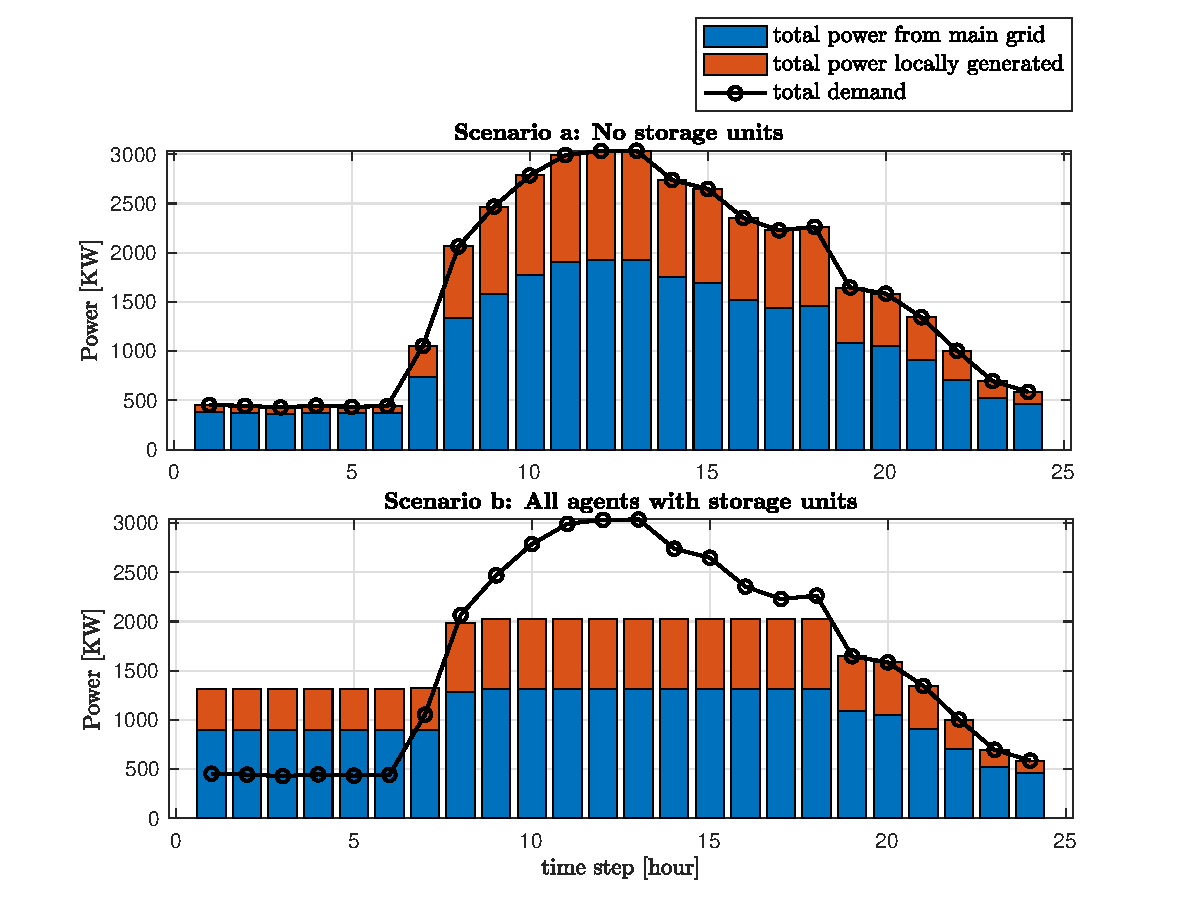
\includegraphics[width=0.6\linewidth]{figures/simB_0402_pt1_v3}
	\caption{	Incorporating storage units causes a peak-shaving effect on the sum of the total power imported from the main grid and the power locally generated.}
\end{figure}
\query[R3-7]{ As a conclusion, the paper presents an interesting mathematical approach for clearing P2P markets. On the another hand, some relevant topics in this area remain uncovered and highlighted as future work. All in all, in my opinion, is a very good work, and should be considered for publication if the issues raised during revision are handled. }
\ans{We thank the Reviewer for the positive comment and recommendation.}

\newpage
\section*{Answers to Reviewer 4}
\textit{This paper presents a mathematical model for a P2P energy market formulated as a generalized game. They introduce in the game a new agent, a Distribution Network Operator (DNO), who is responsible of ensure the operational constraints of the market. Further, they propose a semi-decentralized algorithm to solve the problem, ensuring convergence to a Nash equilibrium. Finally, a numerical study is used to show the relevance of the market framework and the scalability of the algorithm.}


\query[R4-1]{In my opinion, the paper is clearly written, with a detailed explanation of the mathematical aspects, and introduces some relevant results. However, some questions need to be addressed in order to improve the quality of the work.  }
\ans{We thank the Reviewer for the positive comment.}

\textit{Comments and suggestions: }

\query[R4-2]{The authors state that due to the presence of coupling objective and constraints in the formulation, this implies the inapplicability of other decentralized algorithms employed in the literature (lines 54-57, page 2). This is not strictly true, since it is straightforward to reformulate the problem to decompose the objective function, just by replicating the variables avoiding the decomposition, and introduce new complicating constraints to coordinate these variables. Reformulate this sentence. }
\ans{\green{
What we meant is that games with coupling constraints and coupling objectives cannot, in general, be recast as distributed optimization problems, and therefore be solved via decentralized optimization algorithms.
%
In fact, the original market game (1) and the ``decomposed" one, obtained by including local slack variables and coupling constraints to coordinate these variables have different equilibria (see the simple example at the end of the answer). Therefore, social-welfare optimization methods (e.g., ADMM) cannot be straightforwardly used to solve our game-theoretic problem. This is not surprising since variational GNEs and social optima, i.e., the minimizers of the social welfare, are essentially different configurations and coincide only in special cases. To avoid confusion, in the revised paper, we removed the claim of inapplicability.}}

\green{
\textit{Example.} Consider the 2-player aggregative game:
\begin{align*} 
\text{player }1: \quad \min_{u_1 \in \mathbb R}J_1(u_1,u_2) = (u_1+u_2 + 1)^\top u_1,\\
\text{player }2: \quad \min_{u_2 \in \mathbb R} J_2(u_2,u_1) = (u_1+u_2 + 1)^\top u_2.
\end{align*}
Its Nash equilibria can be found in closed form by solving the system of equations obtained by imposing the pseudo-gradient mapping of the game to zero, i.e.,
\begin{equation*}
\left[
\begin{array}{l}
\nabla_{u_1} J_1(u_1,u_2)\\
\nabla_{u_2} J_2(u_1,u_2)
\end{array}
\right]
=
\left[
\begin{array}{l}
2u_1+u_2+1\\
u_1+2u_2+1
\end{array}
\right]
\overset{!}{=}
\left[
\begin{array}{l}
0\\
0
\end{array}
\right],
\end{equation*} 
which yields a unique NE solution: $(u_1^*,u_2^*) = (-1/3,-1/3) $.\\
Now, consider the generalized game
\begin{align*} \
\text{player }1: \quad 
\left\{
\begin{array}{r l}
\displaystyle
\min_{u_1,\sigma_1 \in \mathbb R}& J_1(u_1,\sigma_1) = (u_1+\sigma_1 + 1)^\top u_1,\\
\text{s.t. } & \sigma_1 - u_2 = 0\\
            &  \sigma_2 - u_1 = 0
\end{array}
\right.
\\
\text{player }2: \quad 
\left\{
\begin{array}{r l}
\displaystyle
\min_{u_2,\sigma_2 \in \mathbb R}& J_2(u_2,\sigma_2) = (\sigma_2+u_2 + 1)^\top u_2,\\
\text{s.t. } & \sigma_1 - u_2 = 0\\
            &  \sigma_2 - u_1 = 0
\end{array}
\right.
\end{align*} 
obtained by decomposing the objective functions using the local slack variables $\sigma_1,\sigma_2$ and the extra coupling constraints $\sigma_1 - u_2 = 0, \, \sigma_2 - u_1$. Let us define the Lagrangian functions
\begin{align*}
\text{player }1: \quad \mc L_1(u_1,u_2,\sigma_1,\sigma_2,\lambda_{1,1},\lambda_{1,2}) &= (u_1+\sigma_1 + 1)^\top u_1 + \lambda_{1,1}^\top(\sigma_1 - u_2) + \lambda_{1,2}^\top(\sigma_2 - u_1),\\
\text{player }2: \quad \mc L_2(u_2,u_1,\sigma_2,\sigma_1,\lambda_{2,1},\lambda_{2,2}) &= (u_2+\sigma_2 + 1)^\top u_2 + \lambda_{2,1}^\top(\sigma_1 - u_2) + \lambda_{2,2}^\top(\sigma_2 - u_1),
\end{align*}
The variational GNEs of this modified game can be obtained in closed form by solving the system of equations obtained by stacking the coupled KKT systems of player 1 and 2, with equal dual variables ($\lambda_{1,1}=\lambda_{2,1} := \lambda_1$ and $\lambda_{2,1}=\lambda_{2,2} :=\lambda_2$) \cite{auslender2000lagrangian}, i.e.,
\begin{align*}
\left[
\begin{array}{c}
\nabla_{u_1} \mc L_1(u_1,u_2,\sigma_1,\sigma_2,\lambda_1,\lambda_2)\\
\nabla_{\sigma_1} \mc L_1(u_1,u_2,\sigma_1,\sigma_2,\lambda_1,\lambda_2)\\
\nabla_{u_2} \mc \mc L_2(u_1,u_2,\sigma_1,\sigma_2,\lambda_1,\lambda_2)\\
\nabla_{\sigma_2} \mc \mc L_2(u_1,u_2,\sigma_1,\sigma_2,\lambda_1,\lambda_2)\\
\sigma_1 - u_2\\
\sigma_2 - u_1
\end{array}
\right] =
%
\left[
\begin{array}{c}
2u_1 + \sigma_1 +1 - \lambda_2\\
u_1 +\lambda_1\\
2u_2 + \sigma_2 +1 - \lambda_1\\
u_2 +\lambda_2\\
\sigma_1 - u_2\\
\sigma_2 - u_1
\end{array}
\right] 
\overset{!}{
=}
%
 \mathbf{0},
\end{align*}
which yields v-GNEs of the form $(u_1^*, u_2^*) = (x,-1/2-x)$, with $x \in \mathbb R$.
{\hfill $\square$}
} 

\query[R4-3]{ In the introduction, the authors assert that they extend a preliminary work by including nonlinear operational constraints, which complicate the analysis. However, they consider a linear approximation of power-flow equations (equations (13)). In fact, it seems that the only nonlinear constraint in the model is (15a), although some quadratic terms appear in the objective function. Is there any justification for this? Probably, the statement must be relaxed.  }
\ans{We agree with the Reviewer that the statement can be made clearer. That statement concerns the analysis for algorithm development as we now have a larger set of coupling constraints than that in \cite{belgioioso2020energy}. In order to have an efficient algorithm, we exploit the structure of these constraints in decomposing the problem, thus resulting in Algorithm 1 in the revised manuscript, which is more complicated than \cite[Algorithm 1]{belgioioso2020energy}. Therefore, in the revised manuscript, we have modified the statement as follows:}

\textit{ \edit{``Our market formulation extends our preliminary work \cite{belgioioso2020energy} by including network operational constraints and system operators in the model, which complicate the analysis as we need to exploit the problem structure to derive an efficient algorithm.''}}

\query[R4-4]{ Related to the previous comment, one of the nonlinearities appears in the objective function related to dispatchable units (equation (2)). However, in the numerical studies the parameter $Q_{i}^{di}$ is taken as zero, becoming a linear objective function, and simplifying the model. The same happens with the objective function associated to storage units (equation (4)). Have you tested the effect of these parameters in the model? Further, if these parameters take a positive value, some of the conclusions presented in the numerical study could change. I suggest the authors to analyze this issue.  }
\ans{We thank the reviewer for raising this point. For our proposed algorithm, we have a convergence guarantee for either linear or non-linear objective functions as long as they are locally convex, i.e., convex with respect to local decision variables.In other words, our proposed algorithm works in the case with quadratic local cost functions. Nevertheless, in view of this comment, we have updated the simulations in Section IV-C, where we now use a quadratic cost of dispatchable production, i.e., $Q_{i}^{di}>0$, for all $i \in \mc N^{\mathrm{di}}$, which varies from one unit to another. The results are shown in Figure \red{7}, where we still observe a peak-shaving effect caused by the introduction of storage units. As this manuscript focuses on the distributed clearing mechanism that we propose, we leave an extensive analysis of the effect of different possible objective functions on the clearing outcome as future work.}

\query[R4-5]{The objective function associated to the power traded with the main grid seems not so natural. If the electricity unit price, $c_{h}^{mg}$ in equation (9) is considered linear (instead of quadratic) with respect to the total consumption, this would simplify this term, further becoming (11) a decomposable function. Could the authors elaborate what is the advantage of using a quadratic term here? Is worth the improvement it could add with respect to the difficulty it brings to the model?}
\ans{By the formulation in \red{(9)--(11)}, which is based on \cite{atzeni2013}, the electricity price from the main grid follows a linear inverse demand function where it increases linearly as the total consumption increases. On the other hand, if  $c^{\mathrm{mg}}$ in (9) is a linear function, the electricity unit price is assumed to be constant, which is not the case in the practice. In our view, the former represent better the electricity unit price than the latter, as supported by \cite{atzeni2013noncooperative} and some references therein. In addition, as discussed in \cite[Section II-D]{atzeni2013noncooperative}, the cost function in \red{(11)} can represent either the actual energy cost (as a result of energy generation and transmission costs by the main grid) or simply a pricing function designed to incentivize load-shifting by the end users.}

\query[R4-6]{ Taking into account comment 1, suppose that we consider a reformulation of the problem to avoid coupling objective functions, and we employ the Alternating Direction Methods of Multipliers (ADMM) to solve the P2P market game in (1). Could the authors elaborate if this would be possible? Would the application of the ADDM also guarantees the convergence to a variational GNE of the P2P market game? What are the advantages of using Algorithm 1 proposed in the paper to solve the problem?  }
\ans{\green{Indeed, the only trivial case in which v-GNEs and social optima, i.e., the minimizers of the social welfare, coincide is for games with decoupled objective functions. This fact can be shown, for example, by a direct comparison of their KKT systems. In this special case, the original v-GNE seeking problem and the social welfare minimization problem are equivalent. Hence, the latter can be tackled via existing distributed optimization algorithms, e.g. ADMM. Unfortunately, in general, it is not possible to trivially reformulate games with coupled objectives as optimization problems -- see R4-3 for a simple counter-example in which a straightforward decoupling of the local objective functions fails to preserve the original equilibria. This simple fact motivated many researchers in recent years to design ad-hoc algorithms for games and generalized games with coupled cost functions, see e.g.  \cite{yi2019,paccagnan2019,liang2017distributed, koshal2016distributed,gadjov2020single,belgioioso2020b}.
}
}

\query[R4-7]{ Regarding to the scalability of the algorithms, the author evaluates the convergence of the algorithm with respect to the number of agents and the connectivity, but they do not provide any information about the computational times. This is relevant to evaluate if it could be applied in a real large-scale system. }
\ans{We thank the Reviewer for raising this point. We agree that the computational time is relevant in practice and thus we have added the remark below in the caption of Figure 10. Please, refer to our answer to the comment [R1-7] for a detailed discussion on the applicability of the proposed market-clearing mechanism on real large-scale systems.} %\red{particularly for the simulations with different numbers of agents} 

\textit{\edit{`` The average computation times of the inner loops, i.e., Algorithm~2 and 3, obtained on a computer with Intel Xeon E5-2637 3.5 GHz processors and 128 GB of memory, are 74.5 ms and 1.13 s, respectively.
		''}}
%

 \query[R4-8]{ Given a prosumer $i$, when Algorithm 1 is applied, in order to update the dual variable related to reciprocity constraints, the value of the power traded with neighbors plays an important role. In detail, I mean $\{p^{tr}_{(j,i)}\}_{j\in \mc N_{i}}$, the forward trade estimate to prosumer $i$. It seems that, depending on the order the prosumers are considered, the coordination of these variables could change, so that the convergence of the algorithm. Hence, it could be interesting to analyze how this affect to the behavior of the algorithm. For example, could it benefit to consider first prosumers with less neighbors, since maybe they reach faster an equilibrium? }
 	\ans{\green{
In the proposed market-clearing mechanism, all the local (primal and dual) updates of the prosumers are performed in parallel. We explicitly clarified this point in the new algorithm layout (see the new Algorithm 1).
 	}}
 
 \textit{Minor comments:}
 
 	\query[R4-9]{ The notation used to define the quadratic terms of the objective functions must be introduced previously as “Basic notation”.  }
 	\ans{We thank the reviewer for this suggestion and we have introduced the notation as follows:}
 	
 	\edit{\textit{``Given $x \in \bb R^n$, $\|x\|_A^2 = x^\top A x,$ with square matrix $A \succ 0$.''}}
 	
 	\query[R4-10]{ The references to the lines of Algorithm 1 (in page 7) appearing in the text must be revised. For example, in item (iv) of Remark 2 (page 6), it must appear “…..(lines: 28-31)”. In the box related to dual variable update of prosumer $i$, in Figure 2 (page 6), the line references must be: lines 19-24. }
 	\ans{We thank the reviewer for noticing this errors and we have updated the references to the lines of Algorithm 1 in Remark 2 and Figure 2.}

\bibliographystyle{apalike}
\bibliography{ref}
\end{document}
